% !TeX spellcheck = en_US
\documentclass[a4paper,12pt]{article}

\usepackage{fullpage}
\usepackage{fourier}
\usepackage{amsmath}
\usepackage{color}
\usepackage{graphicx}
\usepackage{titlesec}

\titleformat{\subsection}[hang]{\large\bfseries}{\alph{subsection})\quad}{0pt}{}

\newcommand{\twodo}[1]{\textcolor{red}{\textbf{todo:} #1}}

\title{\textbf{Exercises for Image Processing 1}\\Problem Sheet 3}
\author{Axel Brand\\6145101 \and Nour Elfaramawy\\6517858 \and Konstantin M\"ollers\\6313136 \and Sibel Toprak\\6712316}

\begin{document}
	\maketitle
	
	\section{Perspective Transforms}
	
	\subsection{Straight Line Projection}
	
	A straight line in a 3D scene can be described by the following formula:
	
	\begin{align}\label{eqn:1} \vec{t} = \vec{p} + r \cdot \vec{d},\end{align}
	where $\vec{p}$ is a position vector and $\vec{d}$ is a direction vector. Every possible point on the line $\vec{t}$ can be reached by finding the appropriate $r$.
	
	Furthermore, we can split the equation~\ref{eqn:1} into its components:
	\begin{align}
		t_x &= p_x + r \cdot d_x \\
		t_y &= p_y + r \cdot d_y \\
		t_z &= p_z + r \cdot d_z.
	\end{align}
	
	If we now perform the projection, we obtain the following formulas:
	\begin{align}
		\label{eqn:2} t'_{x} &= t_x \cdot \frac{f}{t_z} \\
		\label{eqn:3}t'_{y} &= t_y \cdot \frac{f}{t_z}\\
		t'_{z} &= f.
	\end{align}
	
	From equations \ref{eqn:2} and \ref{eqn:3} we can conclude a straight line vector specification for a 2D scene:
	
	\begin{align}\label{eqn:4} \vec{s} = \vec{0} + \frac{f}{t_z} \cdot \binom{t_x}{t_y}.\end{align}
	
	Because we were able to construct a 2D straight line formula from any 3D one, we have shown that the obtained 2D projection stays a straight line. $\square$
	
	\subsection{Parallel Line Projection}
	
	In the case of \textbf{Orthographic projection}. Then all lines which are parallel in the real world are also parallel in the projected world.
	
	\subsection{Sphere Projection}
	
	Spheres are looking like ellipses in a 3D projection:
	
	\begin{figure}[h!]
		\centering
		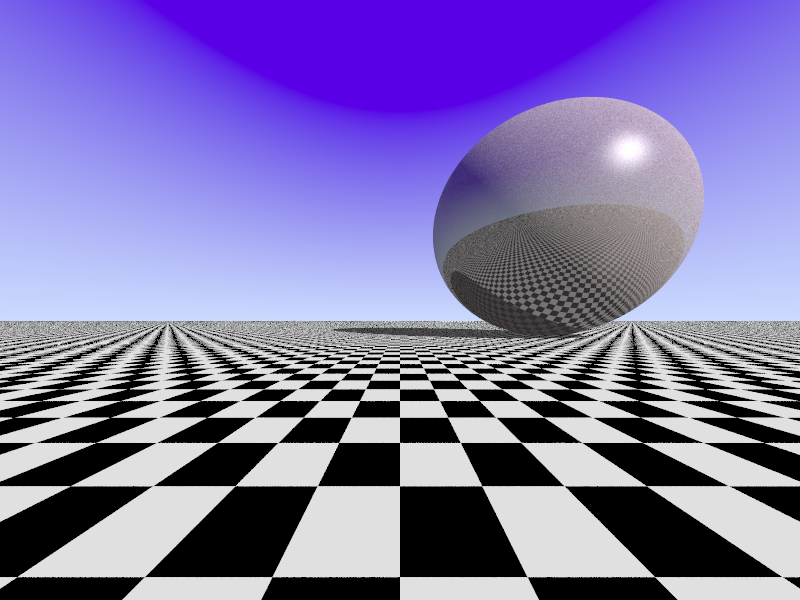
\includegraphics[width=0.7\textwidth]{E03.png}
		\caption{Sphere rendered with perspective projection in POV-Ray.}
	\end{figure}
	
	
\end{document}